\documentclass[Master.tex]{subfiles}

\graphicspath{{images/}}
\begin{document}
%\doublespace
\chapter{Accurate Representation of Phonon Distributions}

\section{Discrete Oscillator Approximation}
  The LEAPR module of NJOY, which is used to prepare thermal scattering data in the form of the scattering law, $S(\alpha,\beta,T)$, often approximates peaks in the phonon spectra as discrete oscillators, and models them as weighted $\delta$-functions. In the event that a user would want to avoid this approximation, and instead apply the continuous phonon distribution treatment to those selected areas, it is crucial to verify agreement between these two methods. To test this, a simplified model for H in H$_2$O is used, which is modeled after Test Problem \#9 in the NJOY 2016 release~\cite{njoy}.
  \subsection{Problem Specifications}\label{sec:test9}
    The test case used for this discrete oscillator discussion depicts a simplified H in H$_2$O model. The water is comprised of H-1 and O-16, and is held at $T=296$ K. An input phonon spectrum is used for the solid-type continuous model, and two discrete oscillators are used to represent higher energy peaks. The phonon distribution and discrete oscillators, which are gotten from Test \#9 in NJOY-2016, are plotted in Fig.~\ref{fig:waterPhonon}~\cite{njoy}. 
  \begin{figure}[h]
    \begin{center}
      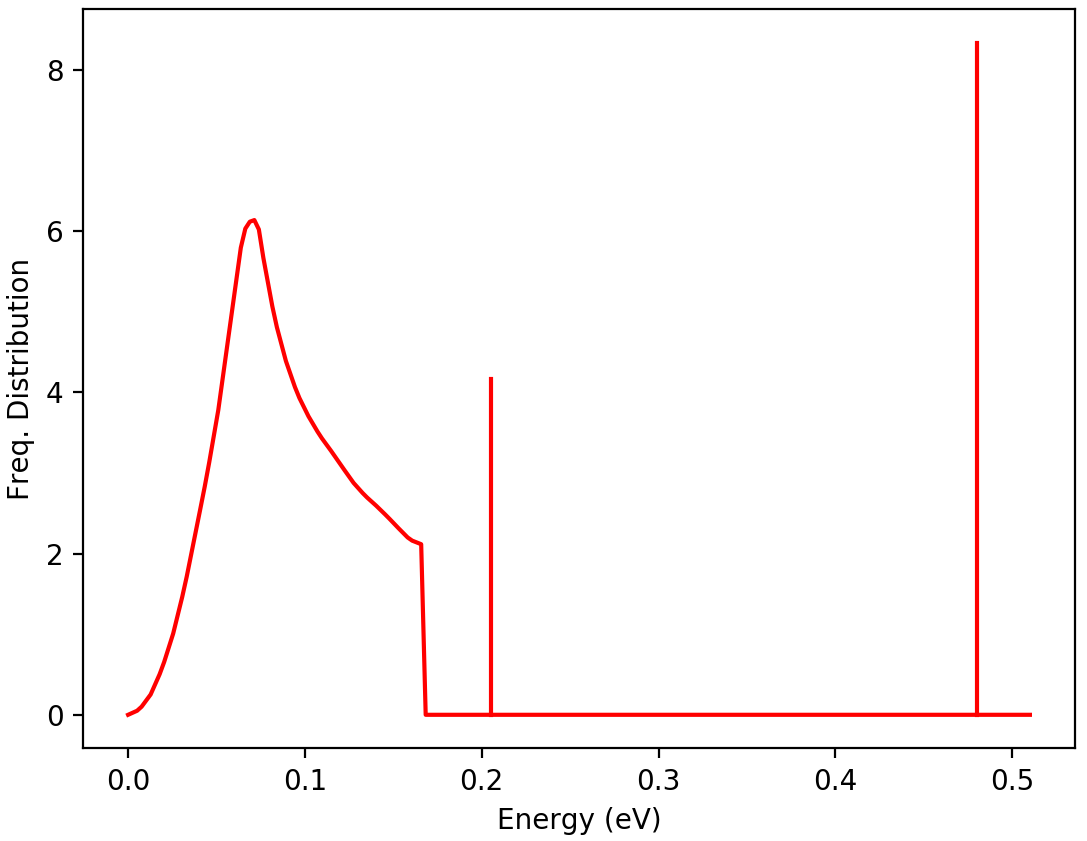
\includegraphics[scale=0.7]{waterPhononDistb}
      \caption[Phonon Distribution for NJOY 2016 Test Problem 9]{The phonon distribution for NJOY 2016 Test Problem 9 is shown above. It contains a continuous contribution, shown on the lower energy region, and two $\delta$ functions to approximate the higher energy peaks. The $\delta$ functions are of arbitrary height relative to the continuous spectrum. }
      \label{fig:waterPhonon}
    \end{center}
  \end{figure}

  The continuous phonon spectrum is defined as $\rho(\beta)=\rho(\Delta E/k_bT)$ for $\Delta E$ spanning from 0-0.16575 eV, where the energy grid is uniformly spaced in increments of 0.00255 eV. No translational/diffusive contribution is considered ($\omega_t=0$). The continuous weighting $\omega_s$ is set to 0.5, and the discrete oscillator energies and weights are provided in Table~\ref{tab:test9_delta_facts}. Note that the listed weights satisfy the normalization requirement stated in Eq.~\ref{eq:weightsSumTo1}.
  %To test this, a simplified version of the NJOY 2016 release Test Problem 9 is considered~\cite{njoy}. The LEAPR component of Test Problem 9 models H in H$_2$O using a slightly simplified phonon spectrum, and moderately coarse $\alpha,\beta$ grids (65 and 75 values, respectively). Fig.~\ref{fig:waterPhonon} contains the phonon spectrum that NJOY 2016 uses in their Test Problem 9. 
  %For Test Problem 9, the continuous region of phonon is defined as $\rho(\beta)=\rho(\Delta E/k_bT)$ for $\Delta E$ spanning from 0-0.16575 eV, where the energy grid is uniformly spaced in increments of 0.00255 eV. The translational contribution to Test Problem 9 is removed $(\omega_t=0)$, and thus the continuous weighting $(\omega_s)$ is increased from 0.444444 to 0.5.  The locations and weights of the two discrete oscillators are provided in Table~\ref{tab:test9_delta_facts}. Note that, as required by Eq.\ref{eq:weightsSumTo1}, 
 % \begin{equation}
 %   \omega_s+\omega_1+\omega_2= 0.5 + 0.166667 + 0.333333 = 1.0.
 % \end{equation}
  \begin{table}[h]
    \centering
    \caption[Energies and Weights for $\delta$ functions used in NJOY 2016 Test Problem 9]{Energies and Weights for $\delta$ functions used in NJOY 2016 Test Problem 9}
    \label{tab:test9_delta_facts}
    \begin{tabular}{ |c|c| }\hline
      Energy (eV)& Weighting\\\hline
      0.205& 0.166667\\\hline
      0.480 & 0.333333 \\\hline
    \end{tabular}\\[1ex]
  \end{table}


  \subsection{Compatible $\alpha,\beta$ Values}
  Recalling the definitions of $\alpha$ and $\beta$ that were stated in Eq.~\ref{eq:alpha} and Eq.~\ref{eq:beta}, respectively, it is apparent that not all $(\alpha,\beta)$ pairs are physically compatible. 
			%\begin{equation}
                        %  \alpha=\frac{E'+E-2\mu\sqrt{E'E}}{Ak_bT}\tag{\ref{eq:alpha}}
			%\end{equation}
			%\begin{equation}
                        %  \beta=\frac{E'-E}{k_bT}\tag{\ref{eq:beta}}
			%\end{equation}
  Setting $\mu=\pm1$ gives the minimum and maximum $\alpha$ values, respectively,
			\begin{equation}
                          \alpha_{max,min}=\frac{E'+E\pm2\sqrt{E'E}}{Ak_bT}.
			\end{equation}
			%\begin{equation}
                        %  \alpha_{max}=\frac{E'+E+2\sqrt{E'E}}{Ak_bT}
			%\end{equation}
                        After defining $E'$ in terms of $\beta$ and rearranging, this becomes 
			\begin{align}
                          \alpha_{max,min}=&\frac{(\beta k_bT + E) + E \pm 2\sqrt{(\beta k_bT + E)E}}{Ak_bT}\\
                          =&\frac{\left(\sqrt{\beta k_bT + E} \pm\sqrt{E}\right)^2}{Ak_bT}
			\end{align}
                        which means that, for a given $\beta$, the valid $\alpha$ range is 
                        \begin{equation}
                          \frac{\left(\sqrt{\beta k_bT + E} -\sqrt{E}\right)^2}{Ak_bT} \leq \alpha\leq \frac{\left(\sqrt{\beta k_bT + E} +\sqrt{E}\right)^2}{Ak_bT}.\label{eq:validAlphaRange}
                        \end{equation}
                        This relationship in Eq.~\ref{eq:validAlphaRange} is plotted in Fig.~\ref{fig:valid_ab_pairs}, where an initial energy $E=1$~eV is assumed, and the scattering material is water at $T=296$ K.
                        \begin{figure}[h]
                          \begin{center}
                            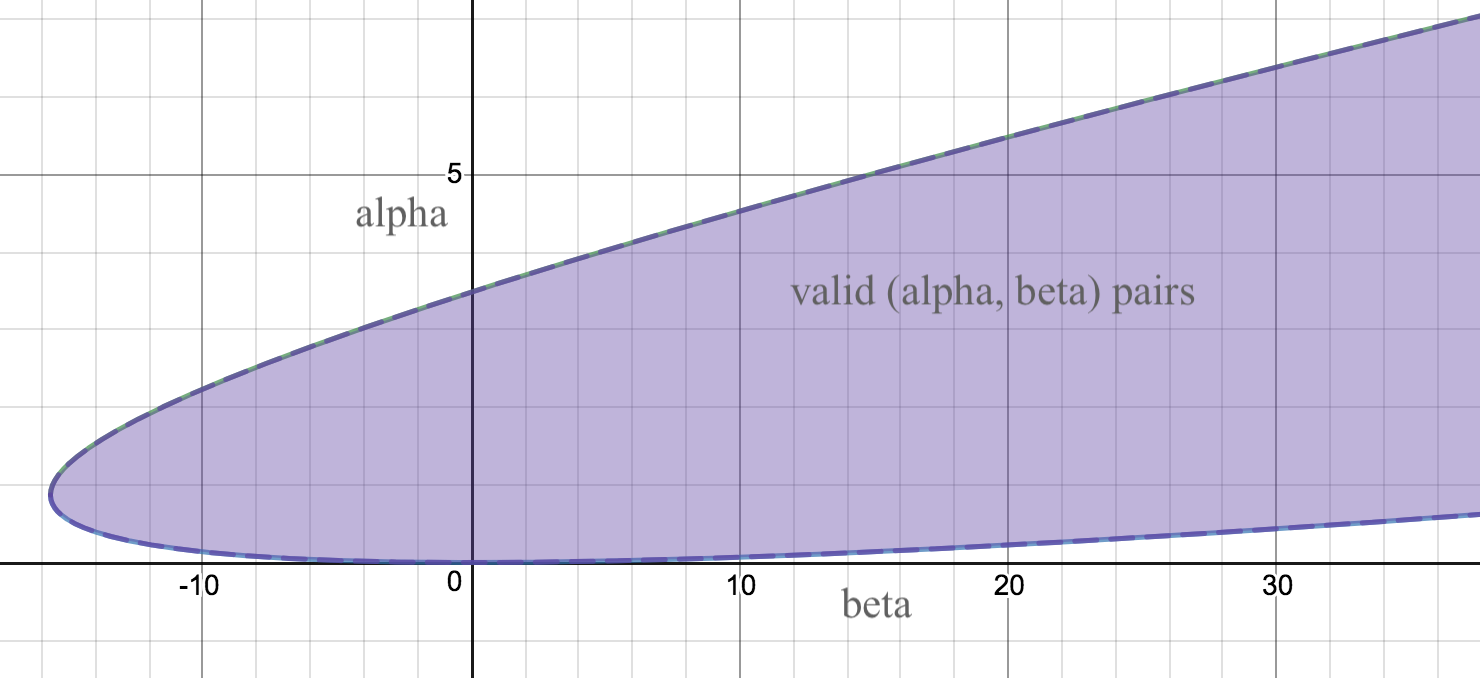
\includegraphics[width=0.7\textwidth]{valid_ab_pairs}
                            \caption[Valid $\alpha$ and $\beta$ values for a 1eV neutron scattering from H$_2$O]{Valid $\alpha$ range, given $\beta$ values, for 1 eV neutron scattering off of water at 296 K. This illustrates the behavior defined in Eq.~\ref{eq:validAlphaRange}.}
                            \label{fig:valid_ab_pairs}
                          \end{center}
                        \end{figure}
                        In all subsequent discussions, only $\alpha$ and $\beta$ values that satisfy the requirement in Eq.~\ref{eq:validAlphaRange} for $E=1$~eV will be presented. This restricts the conclusions to include more physically meaningful values.







\section{Representing Discrete Oscillators as Continuous Points}
  In order to allow users to avoid the $\delta$ function approximation that is commonly used in NJOY's LEAPR module, it is crucial to demonstrate similar behavior between how the solid-type, continuous treatment vs. discrete oscillator treatment processes sharp peaks. The problem specifications detailed in Sec.~\ref{sec:test9} are considered, and the discrete oscillators are represented as thin triangles in the continuous spectrum. To allow for more flexible analysis, LEAPR's source code was translated from Fortran to C++. After presenting the phonon spectra used for the oscillator-triangle analysis, the results of the translated C++ LEAPR vs. legacy Fortran LEAPR are shown, for the simple H in H$_2$O model discussed in Sec.~\ref{sec:test9}.
  %. are compared against legacy Fortran LEAPR for the simple H in H$_2$O model, to establish validity in the method. Then, the discrete oscillators in Test Problem 9 are replaced with triangles of varying thickness, to illustrate that as the thickness of the triangle decreases, it approaches the behavior characteristic of a $\delta$ function oscillator.



  \subsection{Replacing Discrete Oscillator $\delta$ Functions as Triangles}
    To verify that discrete oscillator treatment can be replicated by using increasingly thin triangles, each triangle must integrate to the weight of its corresponding $\delta$ function. Triangles of various widths (2,4,6,8, and 10 grid spaces) are used to replace both $\delta$ functions, and are plotted in Fig.~\ref{fig:waterPhononTriangle}. Additionally, a close-up of the 0.204 eV oscillator region is provided to illustrate a discrepancy between the triangle and oscillator locations.
    \begin{figure}[h]
      \begin{center}
        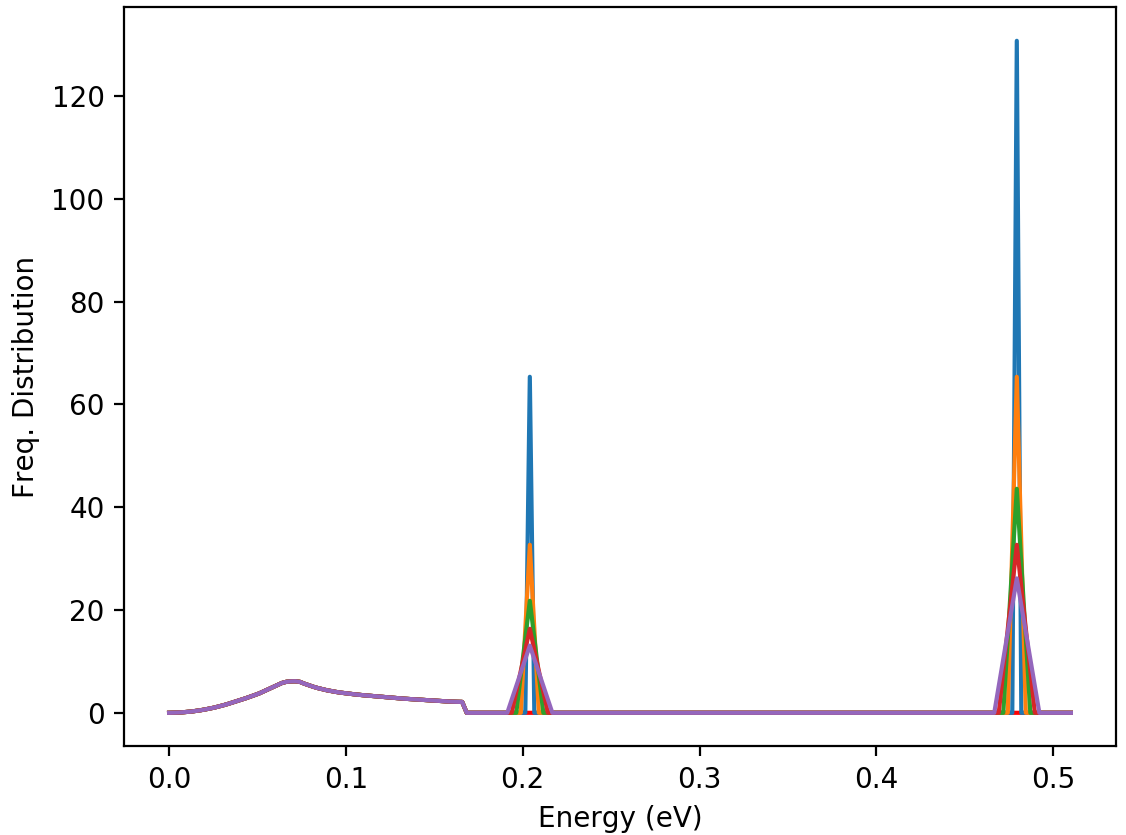
\includegraphics[width=0.49\textwidth]{waterPhononDistTrianglesb}
        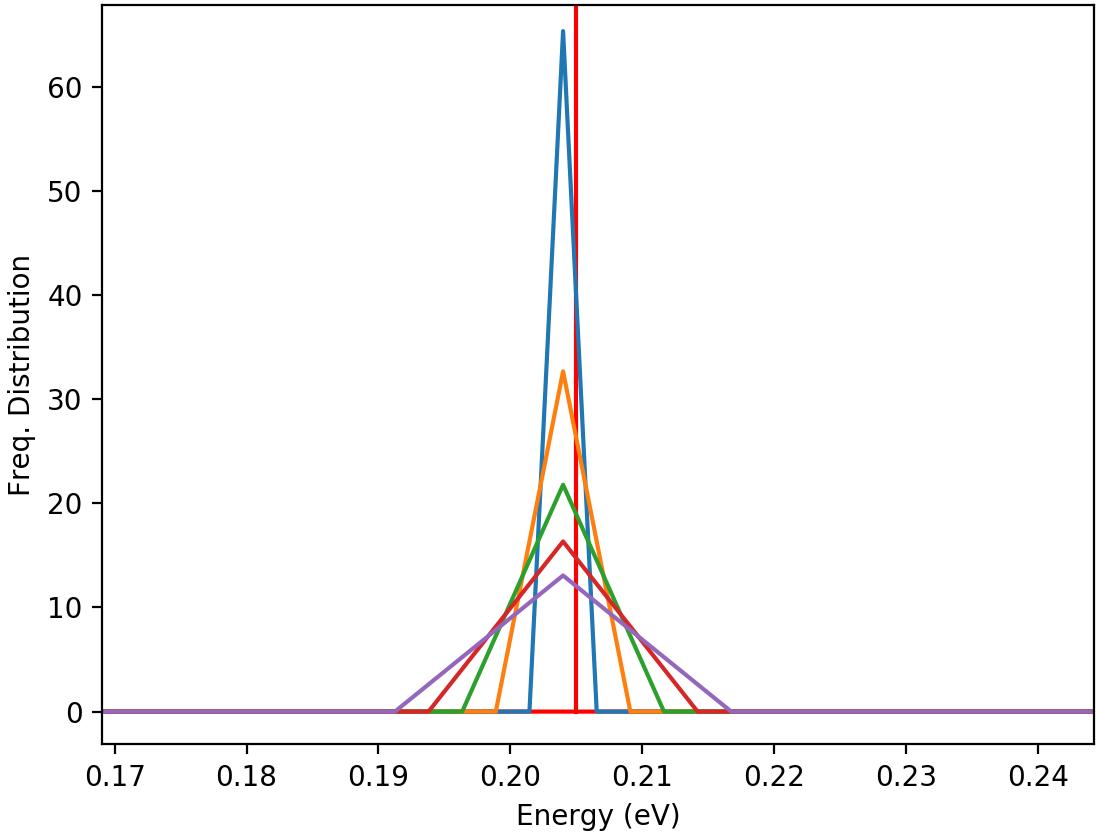
\includegraphics[width=0.49\textwidth]{waterPhononDistTrianglesZoomedb}
        \caption[Triangles of various widths approximating $\delta$ functions for H in H$_2$O]{Phonon Distribution for H in H$_2$O, with oscillators replaced with phonon distribution triangles of various widths. The area under each triangle integrates to its corresponding $\delta$ function weight $\omega_i$, and the lower energy continuous component integrates to the solid-type weight $\omega_s$. A close-up of the 0.204 eV oscillator is provided. Note that due to the continuous spectrum being defined on a uniform grid, the triangles are not perfectly aligned with the $\delta$ function.}
        \label{fig:waterPhononTriangle}
      \end{center}
    \end{figure}
    NJOY requires any continuous phonon distribution to be provided with respect to a uniformly-spaced energy grid. Thus, in Fig.~\ref{fig:waterPhononTriangle}, the centers of the triangles are not necessarily equal to the exact location of the $\delta$ functions that are specified in Table.~\ref{tab:test9_delta_facts}. 
    As a result of the discrepancy between discrete oscillator location and triangle center location, the oscillators energies are shifted slightly to align better with the $\Delta E=0.00255$ eV grid to which NJOY is restricted. The $\delta$ function parameters presented in Table.~\ref{tab:test9_delta_facts} are amended to those in Table.~\ref{tab:amended_delta_facts}.
    \begin{table}[h]
      \centering
      \caption[Energies and Weights for $\delta$ functions, Amended to Align with Energy Grid]{Energies and Weights for $\delta$ functions, Amended to Align with Energy Grid}
      \label{tab:amended_delta_facts}
      \begin{tabular}{ |c|c| }\hline
        Energy (eV)& Weighting\\\hline
        0.204& 0.166667\\\hline
        0.4794 & 0.333333 \\\hline
      \end{tabular}\\[1ex]
    \end{table}
    By slightly shifting the locations of the oscillators so that they are aligned with the triangles' grids, Fig.~\ref{fig:waterPhononTriangle} becomes Fig.~\ref{fig:waterPhononTriangleZoomedShifted}. The oscillator energies detailed in Table~\ref{tab:amended_delta_facts} are the problem specifications used for the remainder of this discussion. 

    \begin{figure}[h]
      \begin{center}
        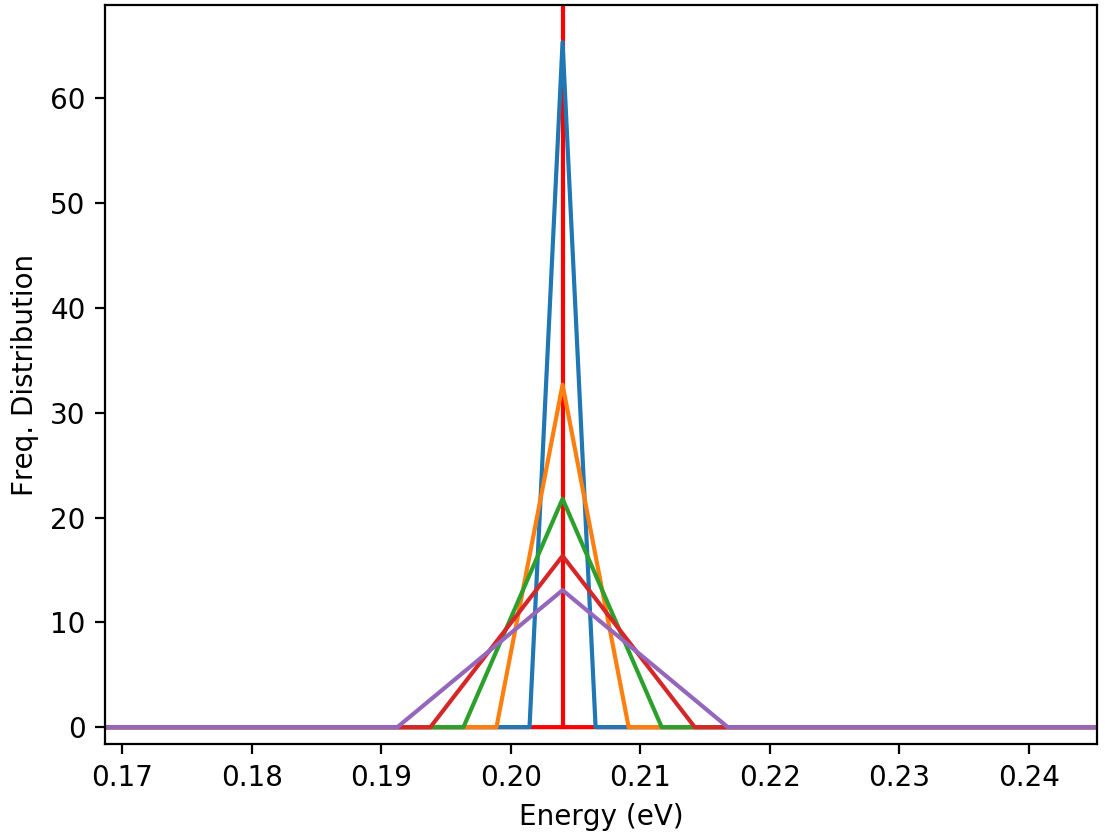
\includegraphics[width=0.49\textwidth]{alteredDeltaZoomedb}
        %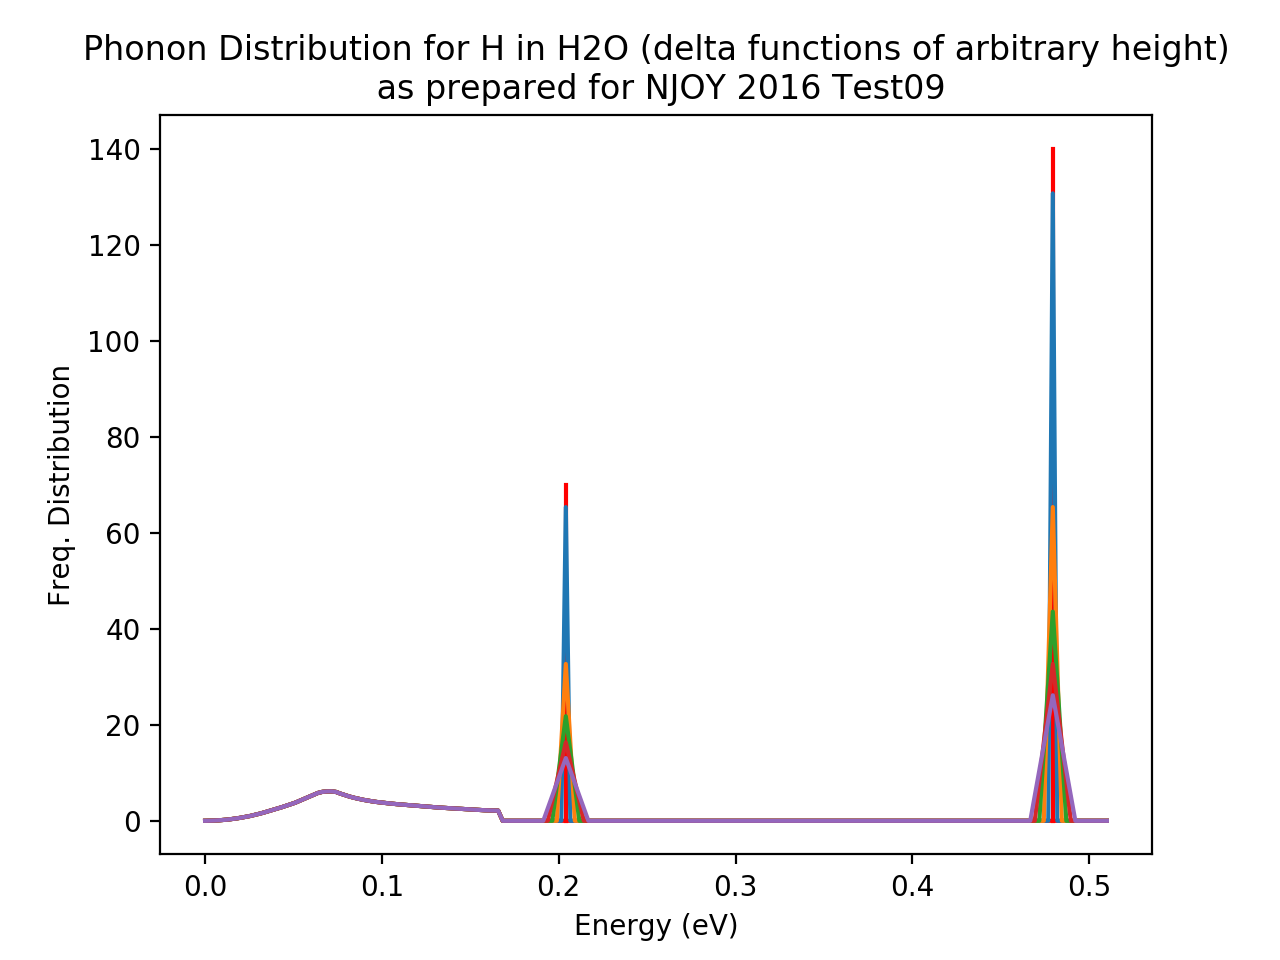
\includegraphics[scale=0.5]{alteredDelta}
        \caption[Triangles of various widths, plotted alongside shifted $\delta$ functions]{Fig.~\ref{fig:waterPhononTriangle} illustrates an offset between the triangle centers and the $\delta$ function location, due to restrictions in the $\rho(E)$ grid. Thus, $\delta$ function locations were shifted to the energies detailed in Table~\ref{tab:amended_delta_facts}.}
        \label{fig:waterPhononTriangleZoomedShifted}
      \end{center}
    \end{figure}






  \subsection{Equivalence of Revised-LEAPR to Legacy-LEAPR}
    NJOY's LEAPR module was translated from Fortran to C++, so as to provide flexibility in later analysis. To use the translated code for analysis requires confidence that it adequately replicates the behavior of the legacy code. To illustrate their compared behavior, Fig.~\ref{fig:me_vs_njoy_sab} contains $S(\alpha,\beta)$ as it was calculated using both the original and the translated LEAPR code. Note that the for nearly all $\alpha,\beta$ values shown, the two datasets are virtually indistinguishable from each other. 
    \begin{figure}[h]
      \begin{center}
        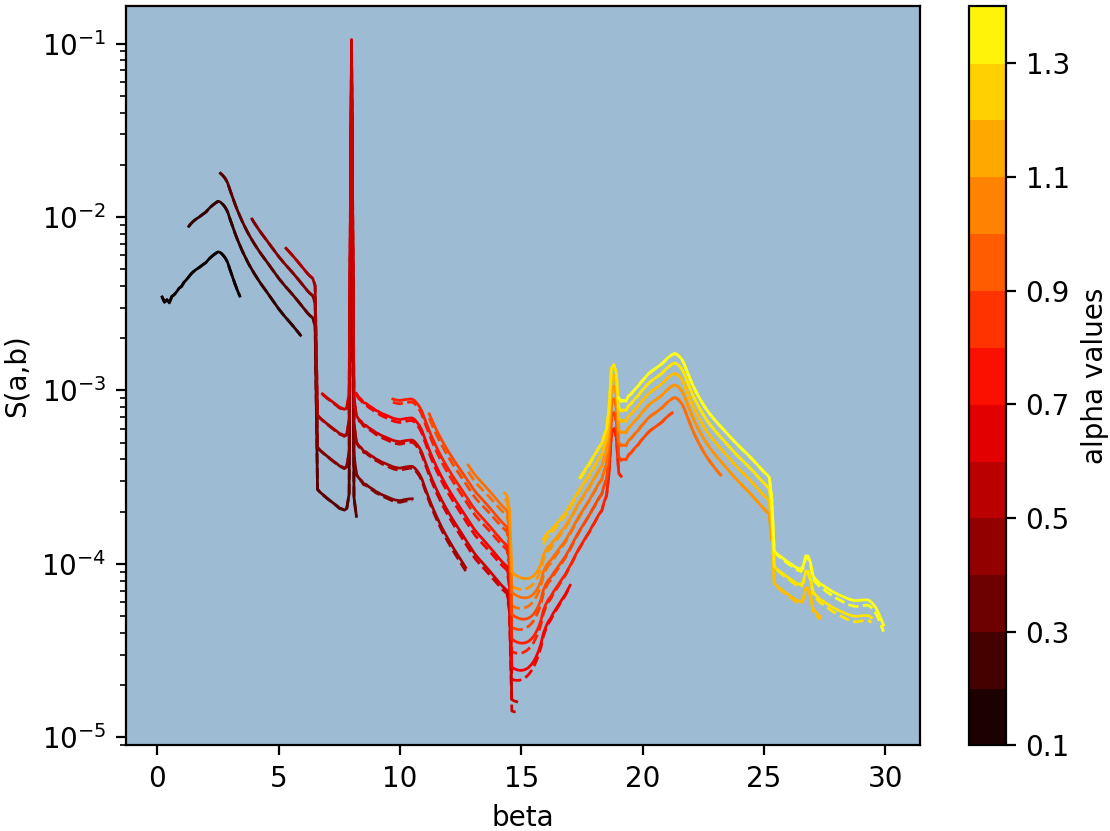
\includegraphics[width=0.85\textwidth]{images/me-vs-njoy-1c}
        \caption[Comparison of Translated vs. Legacy LEAPR, for Test \#9 ($S(\alpha,\beta)$)]{Comparison of Translated vs. Legacy LEAPR, using a simple H in H$_2$O model. Translated and legacy LEAPR are represented using dotted and dashed lines, respectively. Note the sharp peaks that characterize the $S(\alpha,\beta)$ spectrum, which correspond to the summation values in Eq.~\ref{eq:finalDelta}.}
        \label{fig:me_vs_njoy_sab}
      \end{center}
    \end{figure}

    Fig.~\ref{fig:me_vs_njoy_error} shows the percent error between the $S(\alpha,\beta)$ values produced by the translated and original LEAPR, that were plotted in Fig.~\ref{fig:me_vs_njoy_sab}.  Notice that the percent error is significantly lower in the $\beta$ regions where $S(\alpha,\beta)$ is of reasonable size. 


    \begin{figure}[h]
      \begin{center}
        %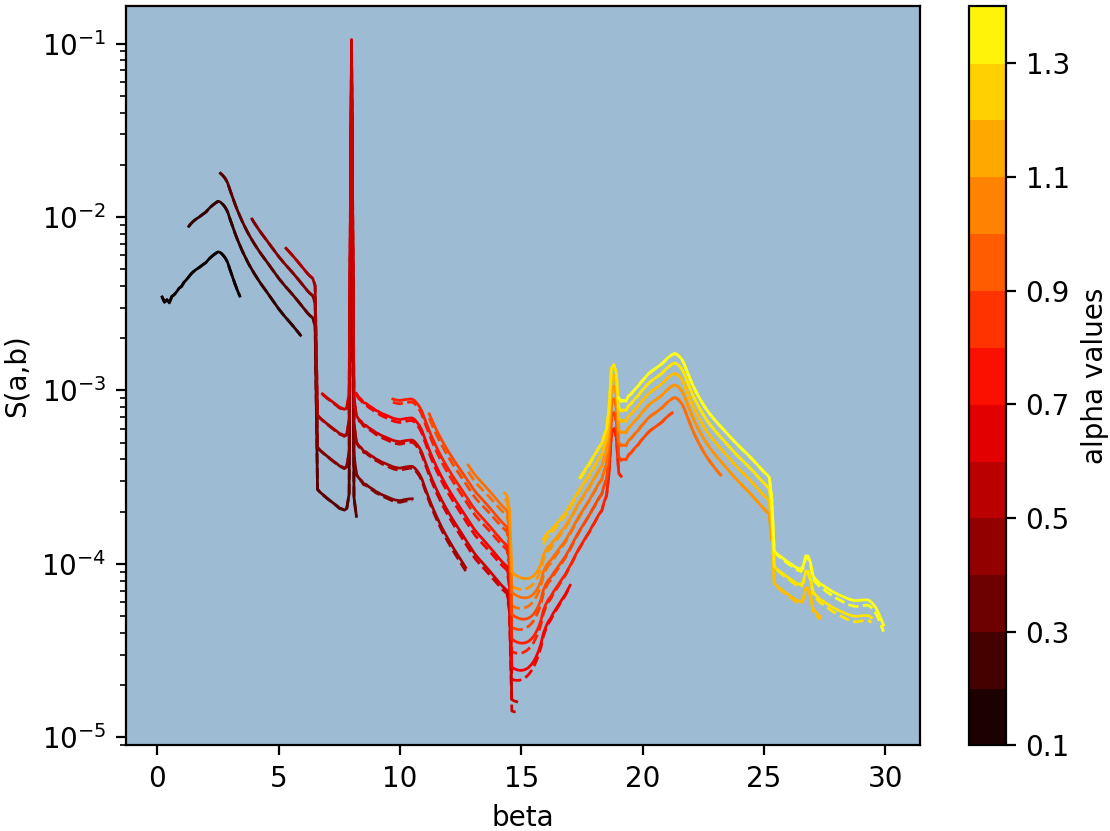
\includegraphics[width=0.70\textwidth]{images/me-vs-njoy-1c}
        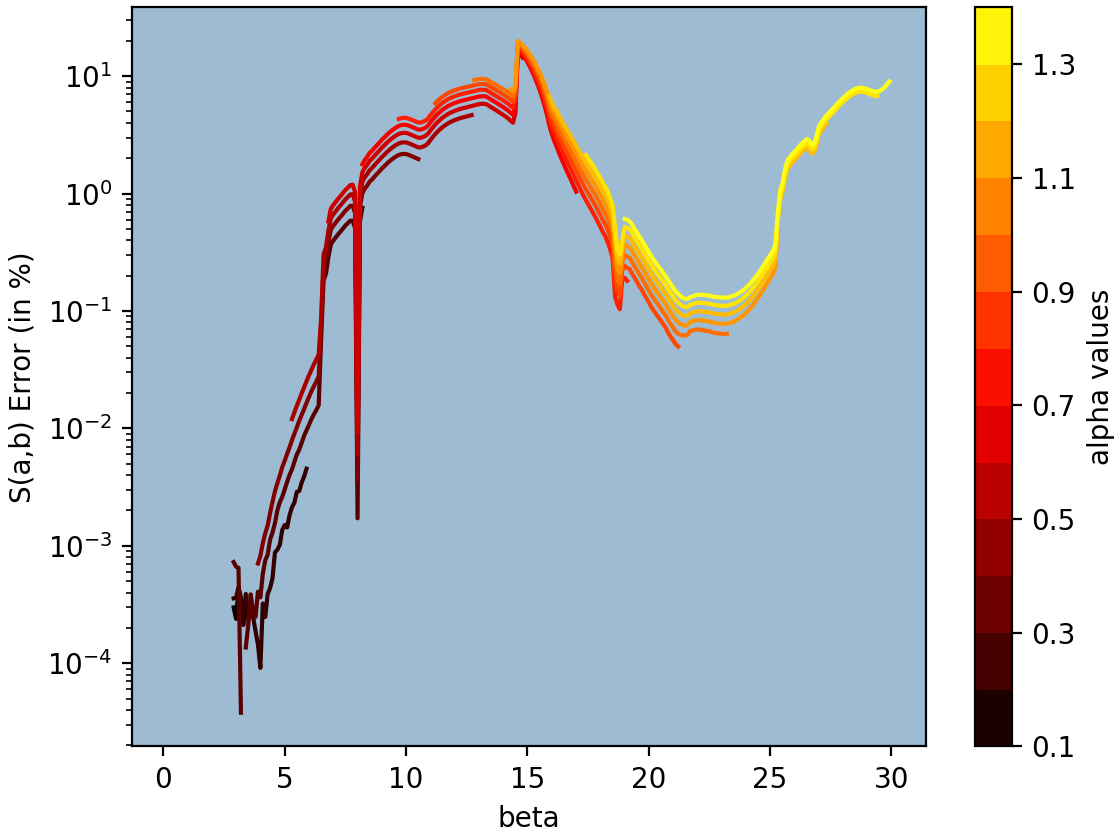
\includegraphics[width=0.75\textwidth]{images/me-vs-njoy-3c}
        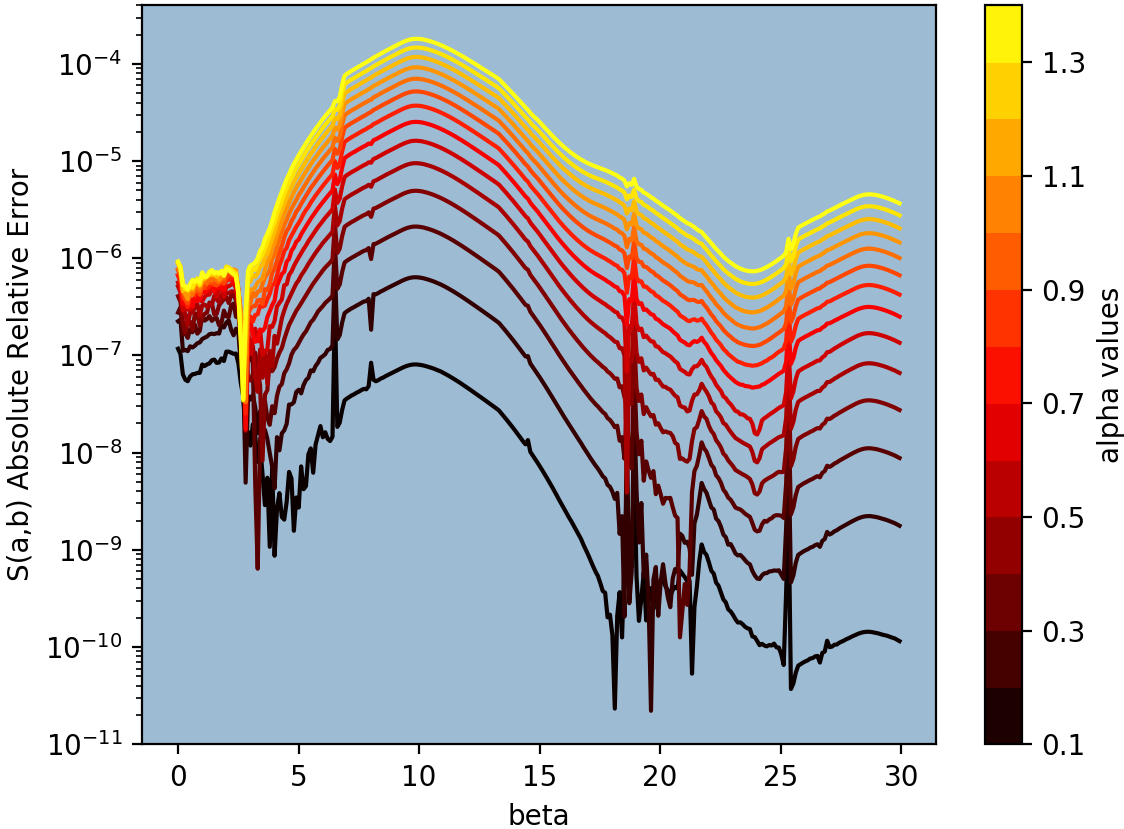
\includegraphics[width=0.75\textwidth]{images/me-vs-njoy-4c}
        \caption[Comparison of Translated vs. Legacy LEAPR, for Test \#9 (\% Error) ]{Comparison of translated vs. legacy LEAPR, for test \#9, with the percent error plotted. Note that in the $\beta$ region where percent error increases, is the same region in Fig.~\ref{fig:me_vs_njoy_sab} where the $S(\alpha,\beta)$ values become significantly smaller.}
        \label{fig:me_vs_njoy_error}
      \end{center}
    \end{figure}



    Thus, the translated version of LEAPR is considered an adequate tool for processing thermal data for the following discussion. However, conclusions drawn using the translated LEAPR will be verified alongside those drawn from the legacy LEAPR. Note that the translated LEAPR was also tested against legacy LEAPR with other cases considered.



    Fig.~\ref{fig:me_vs_njoy_sab} contains many sharp peaks, at $\beta$ values of 7.99, 15.99, 18.79, and 26.79. With the material temperature equal to 296 K, these $\beta$ values can be converted into energy changes in eV, as listed in Table~\ref{tab:spikeLocations}. H

  \begin{table}[h]
    \centering
    \caption[Locations of Peaks in $S(\alpha,\beta)$ Spectrum that Arise From Oscillator Behavior]{Locations of Peaks in $S(\alpha,\beta)$ Spectrum that Arise From Oscillator Behavior. This includes some of the main peaks in Fig.~\ref{fig:me_vs_njoy_sab}, their corresponding values in units of eV (assuming a temperature of 296 K), and the physical reason for the peak. These values arise as a result of Eq.~\ref{eq:finalDelta} where all discrete oscillator combinations are considered in the sums. Here, $E_1$ and $E_2$ correspond to the discrete oscillator energies defined for this problem in Table~\ref{tab:amended_delta_facts}.}
    \label{tab:spikeLocations}
    \begin{tabular}{ |c|c|c| }\hline
      $\beta$ Locations of Peaks& $\Delta E$ Value (eV) & Origin \\\hline
      7.99  & 0.204 & $E_1$ \\\hline
      10.79 & 0.275 & $E_2-E_1$ \\\hline
      15.99 & 0.407 & $E_1+E_1$ \\\hline
      18.79 & 0.479 & $E_2$ \\\hline
      26.79 & 0.683 & $E_1+E_2$ \\\hline
    \end{tabular}\\[1ex]
  \end{table}








\section{$S(\alpha,\beta)$ Response to Continuous vs. Discrete Oscillator Representation} 

  \subsection{$S(\alpha,\beta)$ Response to Thin Triangle vs. Oscillator}\label{sec:thin_triangle_vs_delta}
    The phonon distributions presented in Fig.~\ref{fig:waterPhononTriangle} are input into LEAPR, and the resultant $S(\alpha,\beta)$ is collected. This is compared against the $S(\alpha,\beta)$ grid that is resultant of the typical discrete oscillator representation for the higher end of the H in H$_2$O frequency distribution. As mentioned in Sec.~\ref{sec:test9}, the phonon grid is defined with a uniform energy spacing of $\Delta E=0.00255$  eV, which means that the thinnest triangle available has a total width of $2\times\Delta E=0.0051$ eV. For the remainder of Sec.~\ref{sec:thin_triangle_vs_delta}, this minimum-width triangle will be the only triangle of focus. In Sec.~\ref{sec:vary_triangle_width}, the effects of changing triangle width will be explored.
    Fig.~\ref{fig:sabThinTriangleAllAB} shows the $S(\alpha,\beta)$ grids generated by translated LEAPR, using both the discrete oscillator and the thin triangle phonon representation. The $S(\alpha,\beta)$ grid is plotted against $\beta$ for various $\alpha$ values. There is little discernible difference between the two datasets, so a closeup on the $\beta\approx8$ peak is provided in Fig.~\ref{fig:sabThinTriangleAllABZoomed}.

    \begin{figure}[h]
      \begin{center}
        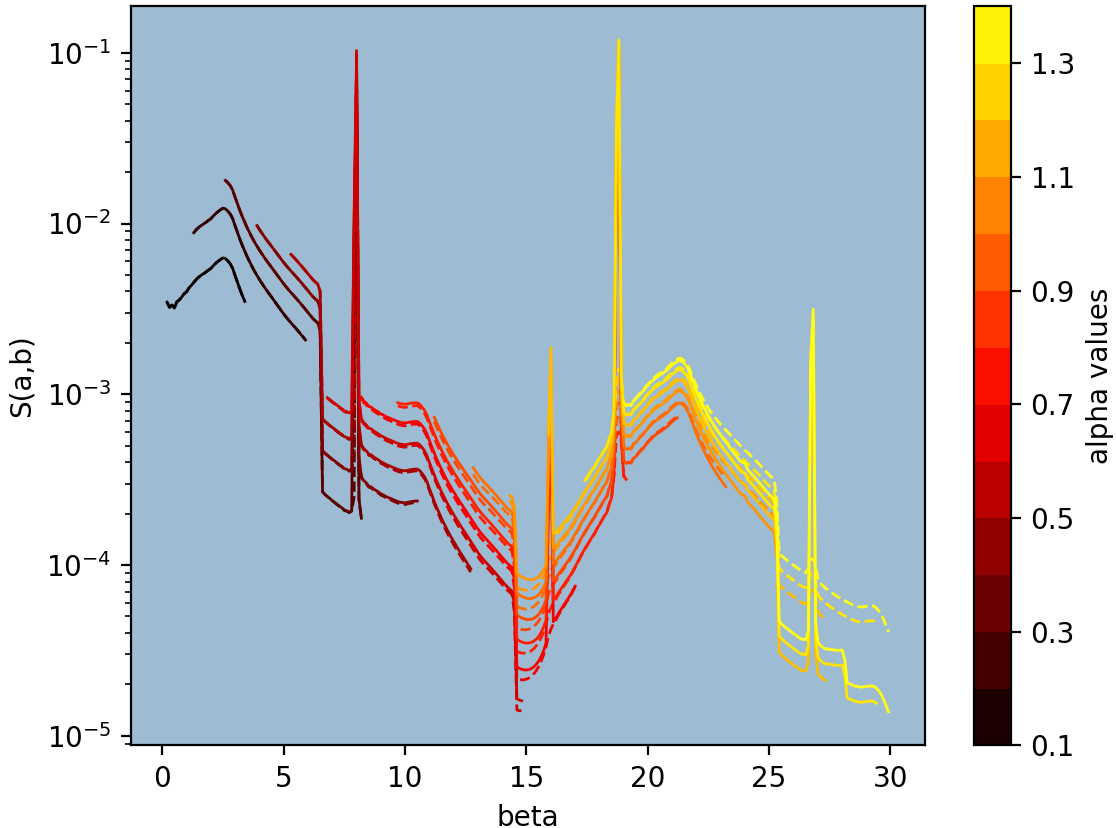
\includegraphics[width=0.7\textwidth]{sab_thinTriangle_and_delta_all_ABb}
        \caption[$S(\alpha,\beta)$ grid, comparing oscillator vs. thin triangle representation (translated LEAPR used)]{$S(\alpha,\beta)$ generated from the translated LEAPR is plotted above, where the discrete oscillator and thin triangle representations are shown using dotted and solid lines, respectively.}
        \label{fig:sabThinTriangleAllAB}
      \end{center}
    \end{figure}



    \begin{figure}[h]
      \begin{center}
        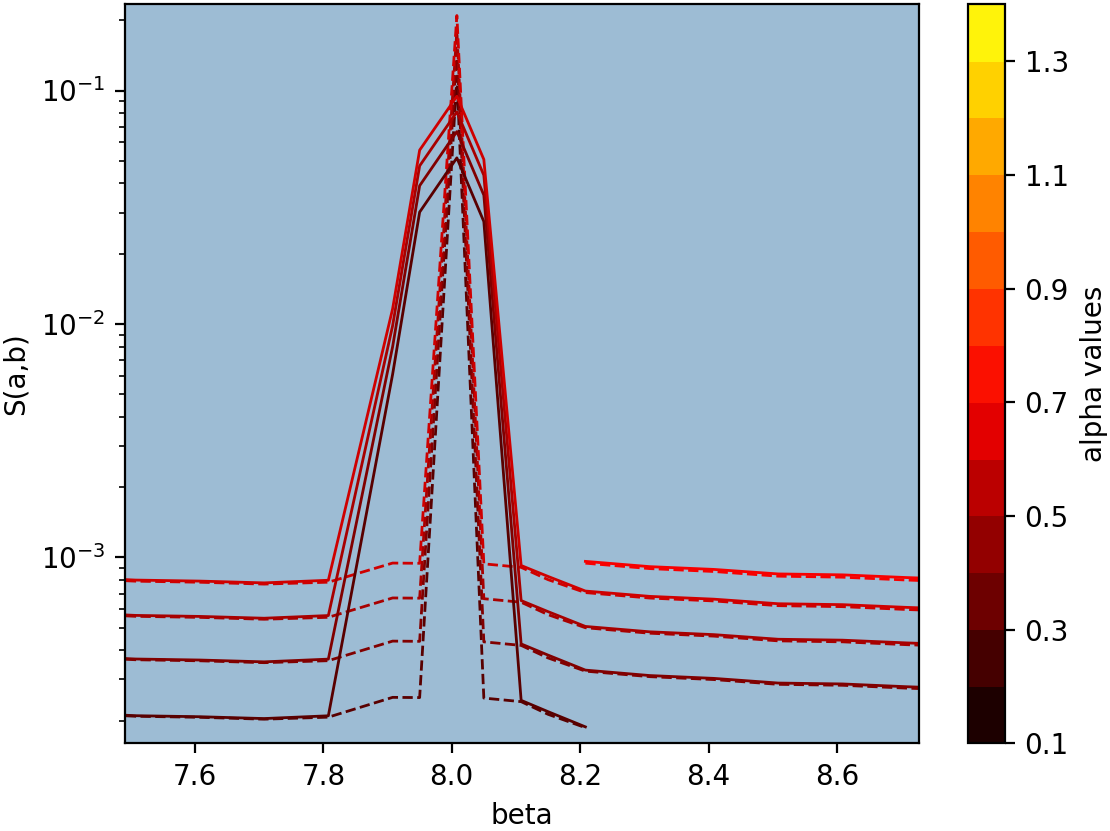
\includegraphics[width=0.7\textwidth]{sab_thinTriangle_and_delta_all_AB_Zoomedb}
        \caption[Close-up view of $S(\alpha,\beta)$ grid that compares oscillator vs. thin triangle representation (translated LEAPR used)]{$S(\alpha,\beta)$ generated from the translated LEAPR is plotted above, where the discrete oscillator and thin triangle representations are shown using dotted and solid lines, respectively. This is a close-up view of Fig.~\ref{fig:sabThinTriangleAllAB}.}
        \label{fig:sabThinTriangleAllABZoomed}
      \end{center}
    \end{figure}
    Looking at Fig.~\ref{fig:sabThinTriangleAllABZoomed}, it is apparent that the continuous representation of the peak has a wider spread than that of the discrete oscillator. This is to be expected, since the triangle needs three points in the frequency distribution to define its shape, while the $\delta$ function is defined at one particular point. 



    %\begin{figure}[h]
    %  \begin{center}
    %    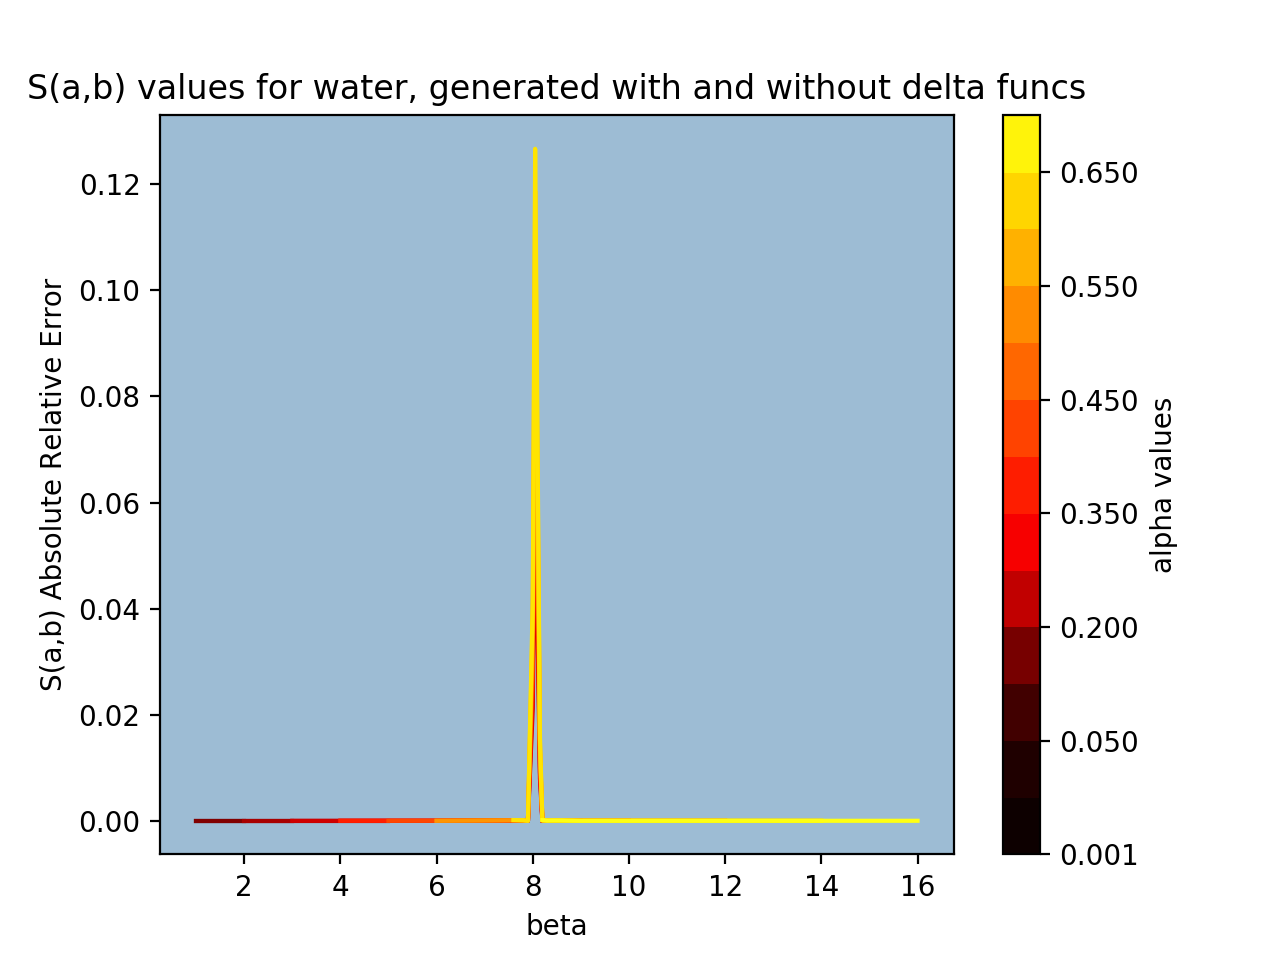
\includegraphics[scale=0.6]{sab_thinTriangle_error}
    %    \caption{This is the absolute relative error between the $S(\alpha,\beta)$ produced using $\delta$ functions and $S(\alpha,\beta)$ produced using a thin (width = 2 spaces) triangle. Note that the error is very small away from the $\beta\approx8.05$ peak. }
    %    \label{fig:sabThinTriangleError}
    %  \end{center}
    %\end{figure}







    
    \clearpage

  \subsection{$S(\alpha,\beta)$ Response to Changes in Triangle Size}\label{sec:vary_triangle_width}



    \subsection*{Results: Triangles of Various Widths vs. $\delta$ Func.}

    \begin{figure}[h]
      \begin{center}
        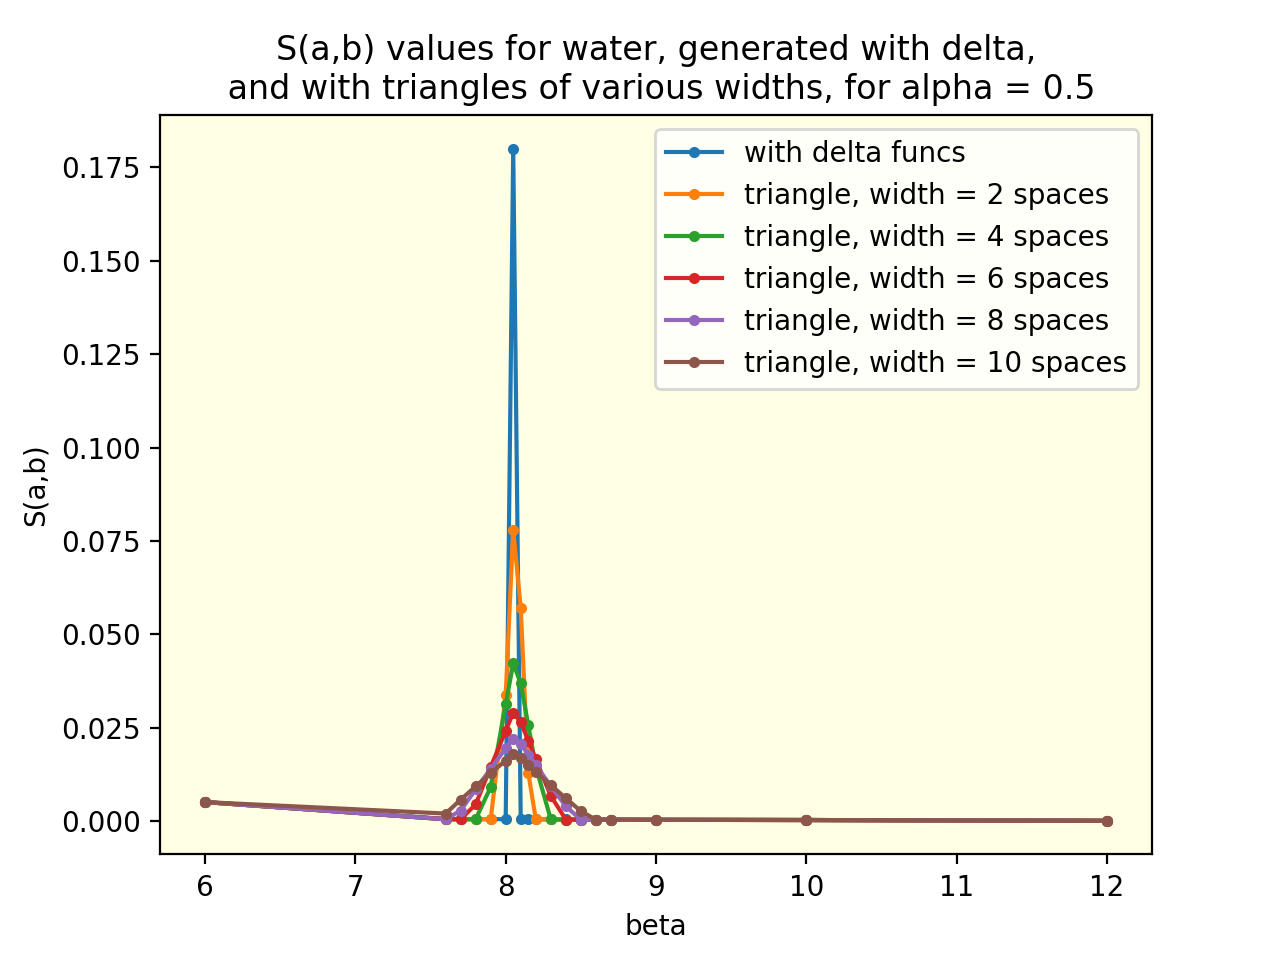
\includegraphics[scale=0.6]{diff_widths_alpha_0p5}
        \caption{}
        \label{fig:diff_widths_alpha_0p5}
      \end{center}
    \end{figure}


    We also look at the total error.
    \[E_{total}=\sum_{\beta}\sum_\alpha \Big|S^\delta(\alpha,\beta)-S^\triangleleft(\alpha,\beta)\Big|\]

    \begin{figure}[h]
      \begin{center}
        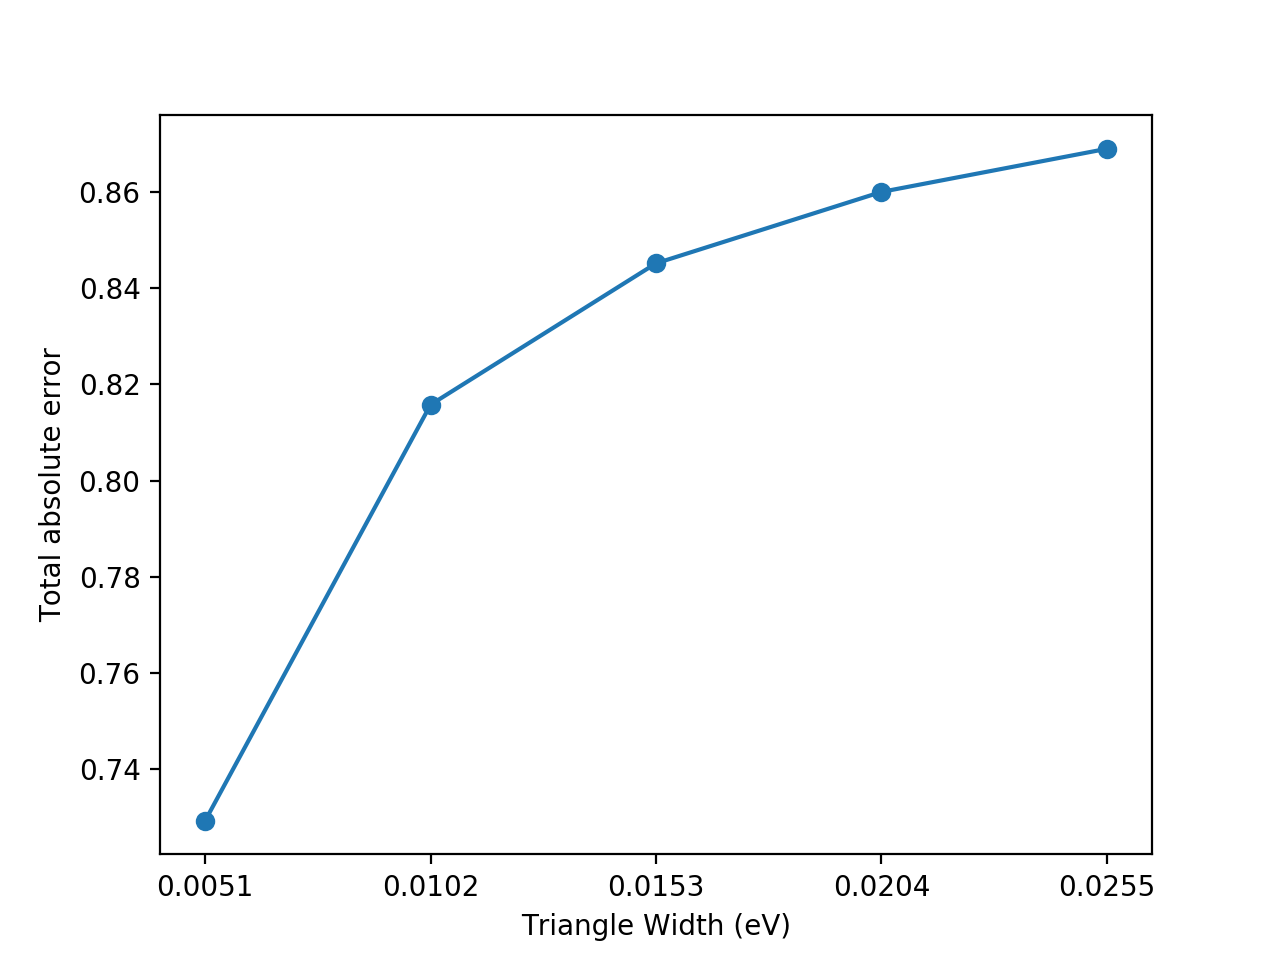
\includegraphics[scale=0.6]{diff_widths_total_error}
        \caption{Note that as the width of the triangle decreases, the total accumulated error decreases significantly.}
        \label{fig:diff_widths_total_error}
      \end{center}
    \end{figure}






          \clearpage
\section{Nonuniform Phonon Distribution Energy Grid}



\end{document}
